\section{Komunikasi Arduino Firmata}
\subsection{Firmata}
	Sebelum Arduino, domain aplikasi berbasis mikrokontroler terbatas programmer perangkat keras. Arduino membuatnya sederhana untuk pengembang yang berasal dari yang lain bidang perangkat lunak dan bahkan untuk komunitas non-coding untuk mengembangkan berbasis mikrokontroler aplikasi perangkat keras. 
	Arduino terdiri dari desain perangkat keras sederhana dengan mikrokontroler dan I / O pin untuk antarmuka perangkat eksternal. Jika seseorang bisa menulis Arduino sketsa yang dapat mentransfer kontrol mikrokontroler dan pin ini ke eksternal mekanisme perangkat lunak, maka itu akan mengurangi upaya seseorang untuk mengunggah sketsa Arduino untuk setiap orang modifikasi. 
	Proses ini dapat dilakukan dengan mengembangkan program Arduino seperti itu kemudian dapat dikontrol menggunakan port serial. Ada protokol yang disebut Firmata, yang tidak persis seperti itu.
	Firmata adalah protokol umum yang memungkinkan komunikasi antara mikrokontroler dan perangkat lunak yang di-host di komputer.
	Perangkat lunak apa pun dari host komputer apa pun yang mampu berkomunikasi serial dapat berkomunikasi dengan mikrokontroler menggunakan Firmata. 
	Firmata memberikan akses lengkap Arduino langsung ke perangkat lunak dan menghilangkan proses memodifikasi dan mengunggah sketsa Arduino. 
	Untuk memanfaatkan protokol Firmata, pengembang dapat mengunggah sketsa yang mendukung protokol ke klien Arduino sebagai proses yang dapat dilakukan sekali pakai. 
	Setelah itu, pengembang dapat menulis perangkat lunak khusus pada komputer host dan melakukan tugas-tugas kompleks. Perangkat lunak ini akan menyediakan perintah melalui port serial ke papan Arduino yang dilengkapi dengan Firmata. Dia dapat terus mengubah logika pada komputer induk tanpa mengganggu perangkat keras Arduino. 
	Praktek menulis sketsa Arduino kustom masih berlaku untuk aplikasi mandiri di mana dewan Arduino harus melakukan tugas secara lokal. Kami akan mengeksplorasi kedua opsi ini di bab-bab yang akan datang.

\subsection{Membaca Data dari Arduino ke MATLAB menggunakan Firmata}
	Firmata dapat membuat kita mengontrol arduino dengan MATLAB tanpa perlu memasukkan program khusus ke dalam arduino. Jadi firmata berfungsi sebagai penyambung agar arduino dapat berkomunikasi menggunakan bahasa pemrograman yang lain.
	
	Untuk melakukannya, berikut ini adalah langkah - langkah atau prosesnya :
		\begin{enumerate}
			\item Instalasi Pustaka Arduino.
				Saat koneksi antara MATLAB dan arduino pertama kali dibangun, disitu MATLAB mengupload pustaka dari firmata ke dalam arduino. Jadi kita harus menginstalasi nya terlebih dahulu.
			\item Koneksikan MATLAB dan Arduino.
				Sesudah menginstalasi pustaka tersebut telah selesai, hubungkan Arduino dan MATLAB menggunakan kabel serial USB. Lalu, check PORT yang Arduino gunakan untuk berhubungan ato berkomunikasi dengan MATLAB. Langkah ini dapat kita cari di dalam Device Manager jika kita menggunakan sistem operasi windows, setelah itu carilah di section PORT(COM&LPT), seperti yang di tunjukkan pada gambar dibawah ini.
				
				\begin{figure}[ht]
					\centerline{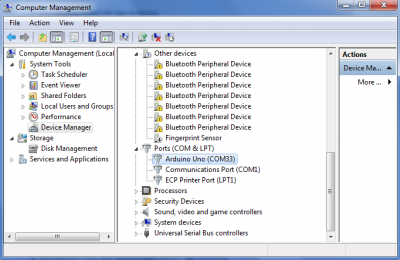
\includegraphics[width=0.5\textwidth]{figures/knksi.png}}
					\caption{Cari PORT yang dipakai Arduino}
					\label{knksi}
				\end{figure}
				
				Setelah itu, ketikkanlah sintaks atau script ini di Command Window dari MATLAB :
				
				\begin{verbatim}
				>> a = arduino
				\end{verbatim}	
				
				Setelah kita menunggu sebentar, MATLAB akan Memberikan respon seperti ini :
				
				\begin{verbatim}
				a = 
 
					arduino with properties:
 
								Port: 'COM33'
								Board: 'Uno'
							AvailableAnalogPins: [0, 1, 2, 3, 4, 5]
						AvailableDigitalPins: [2, 3, 4, 5, 6, 7, 8, 9, 10, 11, 12, 13]
							Libraries: {'I2C', 'SPI', 'Servo'}
				\end{verbatim}
				
				Berdasarkan keterangan yang dipaparkan diatas, dapat kita lihat bahwa jenis arduino yang sedang kita gunakan adalah Arduino UNO, dengan port nya yaitu COM33. Semua pin dan pustaka yang tersedia pun ditampilkan juga di layar. Jangan heran jika komputer anda menunjukkan hasil keterangan yang berbeda, karen semua tergantung jenis papan Arduino anda dan PORT atau COM yang kalian gunakan. Jika kalian sama seperti diatas, kalian dapat mengetikkan script dibawah ini agar lebih cepat.
				
				\begin{verbatim}
					>> a = arduino('com33', 'uno');
				\end{verbatim}
				
				Sekarang kita memakai papan Arduino UNO. Jenis ini telah mempunyai LED  yang telah terpasang di dalamnya. Jika ingin melakuakan testing, gunakan script di bawah ini dan amati lampu LEDnya.
				
				\begin{verbatim}
					>> % menyalakan LED
					>> writeDigitalPin(a,13,1)
					>> % memadamkan LED
					>> writeDigitalPin(a,13,0)
				\end{verbatim}
				
				Kalau sukses kita bisa ke step selanjutnya.
				
			\item Membaca Data dari Arduino.
				Saat praktek, data yang biasa kita dapatkan dari arduino adalah data - data yang didapat dari saat kita menggunakan sensor, bisa digital atau juta analog. Kalian bebas menggunakan yang mana saja, dan kita akan mengirimkan nilai nilai yang terbaca oleh arduino ke MATLAB. Disini yang digunakan adalah potensiometer yang akan mewakili penggunaan sensor analog. Menggunakan ini, akan memudahkan kita dalam mengubah nilai input ke Arduino. Rangkailah seperti gambar di bawah ini. Kaki bagian tengah disambungkan ke pin A0, dan kedua kakinya disambungkan ke GND dan pin 5V.
				
				\begin{figure}[ht]
					\centerline{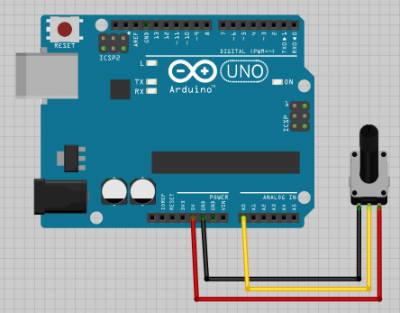
\includegraphics[width=0.5\textwidth]{figures/arduino.png}}
					\caption{Gambar Rangkaian}
					\label{arduino}
				\end{figure}
				
				Kalian bebas memutarnya. Lalu bacalah hasil datanya dengan script readVoltage:
				
				\begin{verbatim}
					>> data = readVoltage(a, 0)
 
					data =
				\end{verbatim}
				Nilai yang sudah didapatkan tadi terkonversi menjadi tegangan 0 - 5V. ADC yang befungsi untuk mengubah sinyal analog menjadi data digital beresolusi 10 bit. Karena itu, data yang didapatkan adalah kira - kira 2^10 = 1024 kemungkinan. Atau dapat juga dihitung seperti berikut ini:
				
				\begin{figure}[ht]
					\centerline{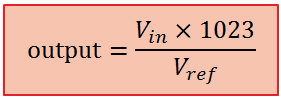
\includegraphics[width=0.5\textwidth]{figures/rumus.png}}
					\caption{Rumus}
					\label{rumus}
				\end{figure}
				
				\begin{verbatim}
					>> outputAnalog = floor((data*1023)/5)
 
					outputAnalog =
						669
				\end{verbatim}
				
				Nilai yang telah kita dapatkan sebelumnya yang sebesar 3.2715 merupakan sebuah data. tegangan referensi kita adalah 5V, dan sintaks floor digunakan untuk membulatkan. Kita dapat melakuakn lebih praktis juka menggunakan sensor yang sebenarnya.
		\end{enumerate}
		
\cite{steiner2009firmata}
